\chapter{Familiarisation with Resistor}
%\ref{sec:background}.

\section{Aim}
%\label{sec:objectives}
	The main objectives are as per following:
	\begin{itemize}
		\tightlist
		\item Explain the function and unit of Resistor
		\item Measure the value of a Resistor
		\item Measure the Tolerance of a Resistor
		\item Explain the types of Resistors
	\end{itemize}

\section{Apparatus}
%\label{sec:objectives}
\begin{itemize}
	\tightlist
	\item Metal-Film Resistor (220 $\Omega$)
	\item Carbon-Film Resistor (220 $\Omega$)
	\item Wire-wound Resistor (10k $\Omega$)
	\item Potentiometer (10k $\Omega$)
\end{itemize}


\section{Theory}
	A resistor is a passive two-terminal electrical component that implements electrical resistance as a circuit element. In electronic circuits, resistors are used to reduce current flow, adjust signal levels, to divide voltages, bias active elements, and terminate transmission lines, among other uses. High-power resistors that can dissipate many watts of electrical power as heat, may be used as part of motor controls, in power distribution systems, or as test loads for generators. Fixed resistors have resistances that only change slightly with temperature, time or operating voltage. Variable resistors can be used to adjust circuit elements (such as a volume control or a lamp dimmer), or as sensing devices for heat, light, humidity, force, or chemical activity.
	
	\subsection{Types of Resistors}
		\begin{figure}[h]
			\centering
			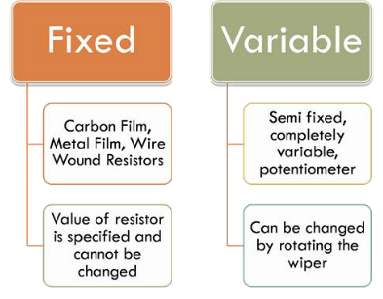
\includegraphics{img/exp1/fig1}
			\caption[Types of Resistor]{}
			\label{fig:typesOfResistors}
		\end{figure}

		\subsubsection{Carbon Film Resistors (Figure \ref{fig:typesOfResistors2}a)}
			\begin{itemize}
				\tightlist
				\item Most general purpose, cheap resistor
				\item Tolerance of Resistance value is usually +/- 5\%
				\item Power ratings of 1/8 W ,1/4 W and ½ W are usually used
				\item Con: Tend to be electrically noisy
			\end{itemize}
		\subsubsection{Metal Film Resistors (Figure \ref{fig:typesOfResistors2}b)}
			\begin{itemize}
				\tightlist
				\item Used when higher tolerance is needed, i.e. more value.
				\item They have about +/- 0.05\% tolerance
			\end{itemize}
		\subsubsection{Wire Wound Resistors (Figure \ref{fig:typesOfResistors2}c)}
			\begin{itemize}
				\tightlist
				\item A wire wound resistor is made of metal resistance wire, and because of this they can be manufactured to precise values
				\item Also, high wattage resistors can be made by thick wire material
				\item Wire wound resistors in a ceramic case are called as ceramic resistors
			\end{itemize}
		\begin{figure}[h]
			\centering
			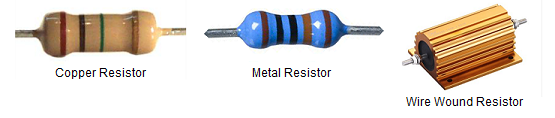
\includegraphics[height=2.5cm]{img/exp1/fig5}
			\caption[Types of Resistor]{}
			\label{fig:typesOfResistors2}
		\end{figure}


\section{Procedure}
	\subsection{Reading Value of Fixed Resistors}
		Resistors are color-coded as they are too small for the value to be written on them.
		There are 4 or 5 bands of color . Value of a Resistor is decoded from these band of colors. (Refer Figure \ref{fig:bands:1} and \ref{fig:bands:2})
		\begin{figure}[ht]
			\centering 
			\subfloat[Band coding on resistors]{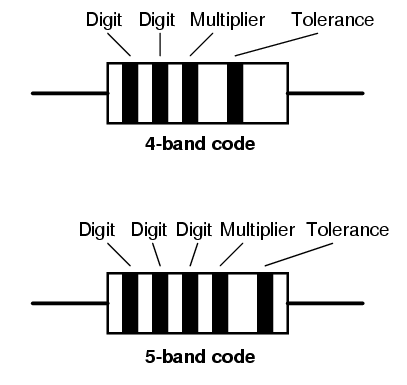
\includegraphics[width=0.3\textwidth]{img/exp1/fig2_1}
				\label{fig:bands:1}}
			\hfill
			\subfloat[4-band/5-band resistors]{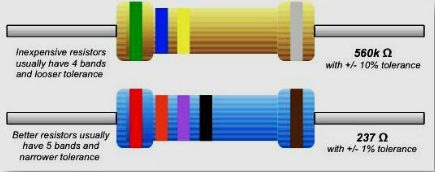
\includegraphics[width=0.6\textwidth]{img/exp1/fig2}
				\label{fig:bands:2}}
			\vfill
			\subfloat[Correct method to hold resistor]{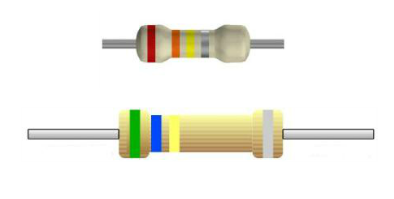
\includegraphics[width=0.3\textwidth,valign=c]{img/exp1/fig4}
				\label{fig:steps:1}}
			\hfill
			\subfloat[Resistor Value table]{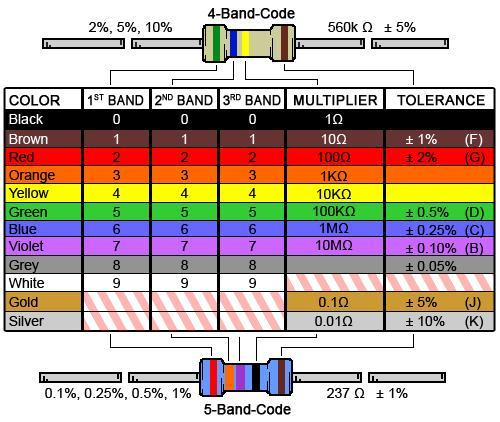
\includegraphics[width=0.6\textwidth,valign=c]{img/exp1/fig3}
				\label{fig:steps:2}}
			\caption{\textit{Resistors have bands on them, showing the resistor value and tolerances in a color-coded format.}}
		\end{figure}
		
		\subsubsection{Procedure}
			\begin{enumerate}
				\tightlist
				\item If your resistor has four color bands, turn the resistor so that the gold or silver band is on right hand side or the end with more bands should point left. (see Figure \ref{fig:steps:1})
				\item The first band is now on the left hand side. This represents the first digit .Based on the color make a note of the digit (Figure \ref{fig:steps:2}).
				\item The second band represents the second digit. The colors represent the same numbers as did the first digit (Figure \ref{fig:steps:2})
				\item The third band divulges how many zeros to add/divide to the first two numbers – for a 4 band Resistor (Figure \ref{fig:steps:2})
				\item The third band denotes the 3rd digit – for a 5 band Resistor (Figure \ref{fig:steps:2}).
			\end{enumerate}
			
			\subsubsection{Tolerance}
			The last band denotes the tolerance . So the value of the 4 band resistor it is +/- 5\% while for the 5 band resistor it is +/- 1\%.
			\begin{itemize}
				\item Tolerance of a Resistor is also an important property to consider .
				\item A 100 ohm resistor with a 10 \% tolerance can mean its value can be any fixed value between 90 to 110 Ohms.
				\item A 120 Ohm resistor with a 10 \% tolerance can mean its value can be any fixed value between 108 and 132 Ohms.
				\item So there is some overlap between 100 Ohm and 120 Ohm resistance in terms of its limits.
			\end{itemize}	

\section{Conclusion}
Resistors are common elements of electrical networks and electronic circuits and are ubiquitous in electronic equipment. The electrical function of a resistor is specified by its resistance: common commercial resistors are manufactured over a range of more than nine orders of magnitude. The nominal value of the resistance falls within the manufacturing tolerance, indicated on the component.